\documentclass[a4paper]{article}

% Set for specific document
\def\DOCTITLE{CSC3621 Coursework 1 Exercise 3}
\def\DOCAUTHOR{Dan Nixon (120263697)}
\def\DOCDATE{16/10/2015}

% Set document attributes
\title{\DOCTITLE}
\author{\DOCAUTHOR}
\date{\DOCDATE}

\usepackage{fullpage}
\usepackage{scrextend}
\usepackage{titlesec}
\usepackage{fancyhdr}
\usepackage[section]{placeins}

% Handle graphics correctly
\ifx\pdftexversion\undefined
\usepackage{graphicx}
% \usepackage[dvips]{graphicx}
\else
\usepackage[pdftex]{graphicx}
\DeclareGraphicsRule{*}{mps}{*}{}
\fi

% Setup headers and footers
\pagestyle{fancy}
\lhead{}
\chead{\DOCTITLE}
\rhead{}
\rfoot{\DOCDATE}
\cfoot{\thepage}
\lfoot{\DOCAUTHOR}

% Set header and footer sizes
\renewcommand{\headrulewidth}{0.4pt}
\renewcommand{\footrulewidth}{0.4pt}
\setlength{\headheight}{15.2pt}
\setlength{\headsep}{15.2pt}

\begin{document}

\section{One time pad encryption program}

The one time pad program is split between pad generation
(\texttt{OneTimePadGenerator.java}) and encryption/decryption
(\texttt{OneTimePadEncryption.java}). The program is used through a command line
interface implemented in \texttt{OneTimePadApp.java} with the following
arguments:

\begin{description}
  \item[\texttt{--generate-pad-file FILE}]
    Generate a pad and save it as \texttt{FILE}.
  \item[\texttt{--length N}]
    Set the length of the generated pad to be \texttt{N} bytes.
  \item[\texttt{--seed N}]
    Sets the seed of the pad generator to \texttt{N} otherwise the seed is set
    by equation \ref{eq:clock_seed}.
  \item[\texttt{--encrypt}]
    Encrypt a message file.
  \item[\texttt{--decrypt}]
    Decrypt an encrypted message.
  \item[\texttt{--pad-file FILE}]
    The pad file to use during encryption or decryption.
  \item[\texttt{--message-file FILE}]
    The message file to be encrypted.
  \item[\texttt{--cipher-file FILE}]
    The file to read/save the cipher to/from.
\end{description}

\subsection{Pad file generation}

Generation of the one time pad is done by generating a random array of bytes
using the \\ \texttt{java.security.SecureRandom} random number generator using a
byte array of length 8 (determined by the value of a long integer) as the seed.

This generator is implemented as the \texttt{generateOneTimePad(int, int)}
method in the \texttt{OneTimePadGenerator} class. There is also a
\texttt{generateOneTimePad(int)} method that only takes the length of the pad as
a parameter, in this case the system clock is used for the seed.

Figure \ref{fig:generate_pad} shows the result of generating a 1MB one time pad
using a set integer key and the first 240 bytes of the hex dump of the generated
pad file.

\begin{figure}[h!]
  \centering
  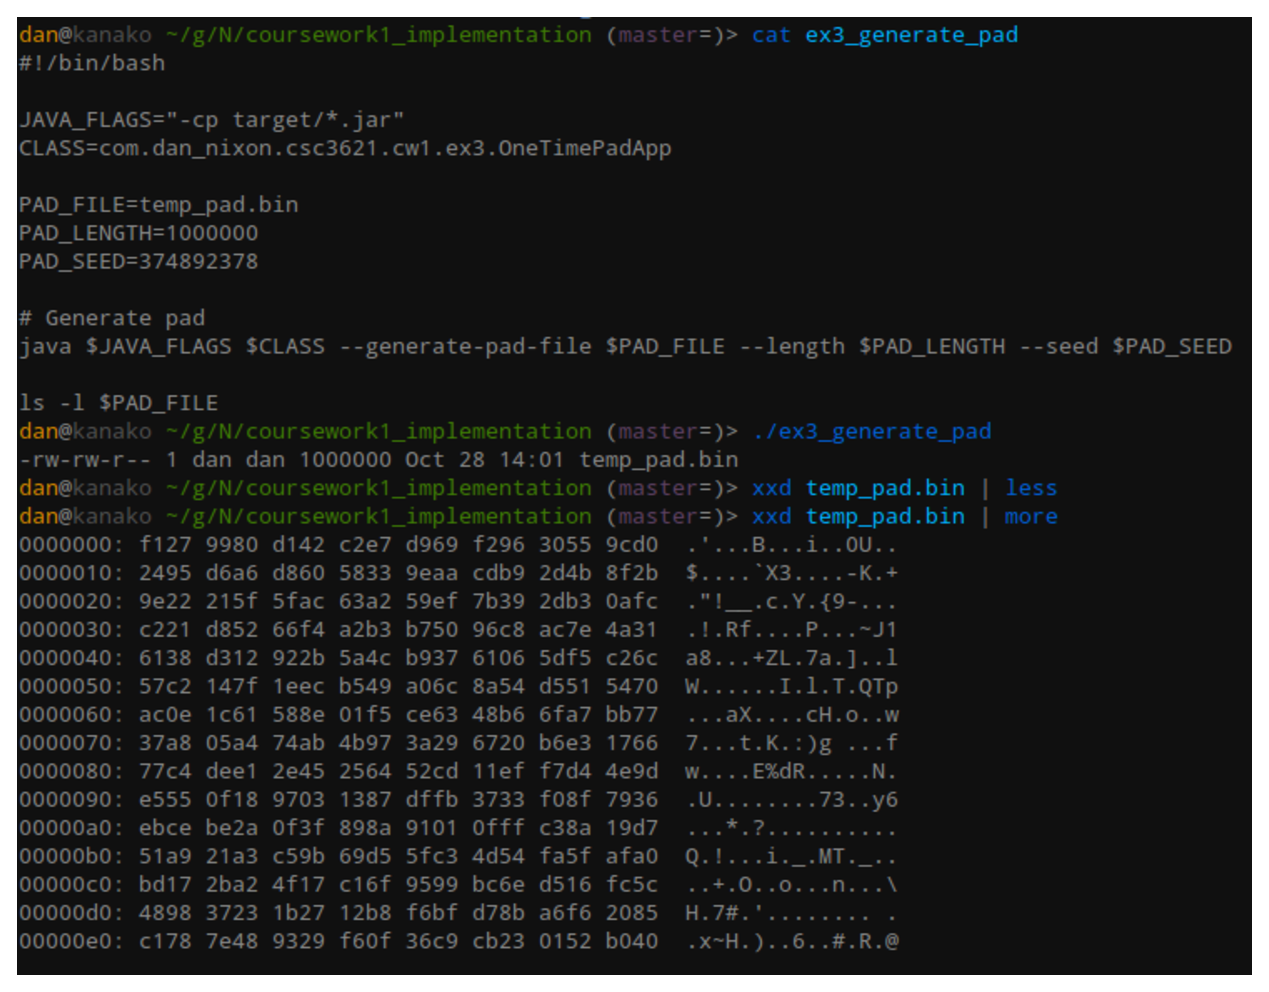
\includegraphics[width=0.75\textwidth]{graphics/ex3_pad_generation.eps}
  \caption{Generation of a one time pad}
  \label{fig:generate_pad}
\end{figure}

\subsection{Encryption and decryption}

Once the pad has been generated encryption and decryption are simple XOR
operations over the pad and message/cipher text arrays (equations
\ref{eq:encrypt} and \ref{eq:decrypt} respectively).

\begin{equation}
  C_{i} = P_{i} \oplus M_{i}
  \label{eq:encrypt}
\end{equation}
\FloatBarrier

\begin{equation}
  M_{i} = P_{i} \oplus C_{i}
  \label{eq:decrypt}
\end{equation}
\FloatBarrier

where $M$ is the plain text message, $P$ is the one time pad and $C$ is the
cipher text.

This functionality is implemented in the \texttt{OneTimePadEncryption} Java
class, specifically the \texttt{encrypt()} and \texttt{decrypt()} methods.

\subsection{Correctness}

The correctness of the encryption and decryption operations is tested using a
unit test in the \\ \texttt{OneTimePadEncryoptionTest.java} file, amongst other
tests this tests the encryption and decryption of the test vector given in the
specification to validate the two operations.

In addition to this I also performed a encryption and decryption cycle on the
plain text from exercise 1 to ensure that a sample of plain text survives the
encryption/decryption cycle intact.

The result of this are shown in figure \ref{fig:enc_dec_cycle}.

\begin{figure}[h!]
  \centering
  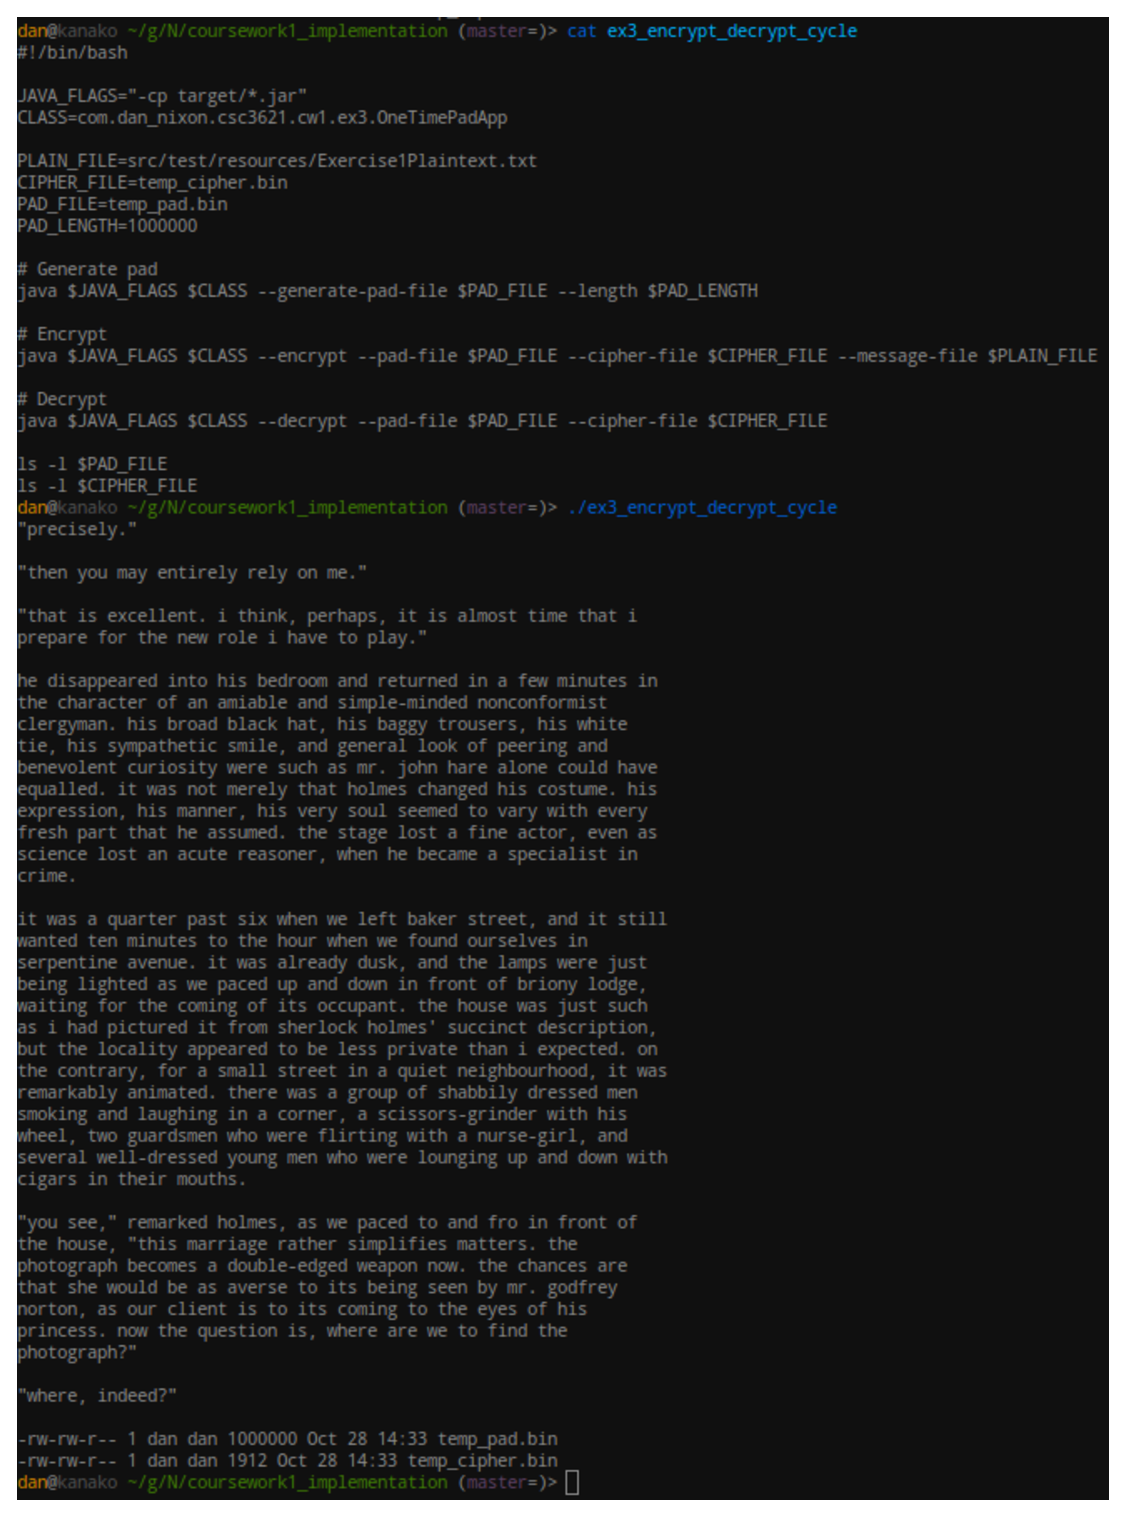
\includegraphics[width=0.75\textwidth]{graphics/ex3_enc_dec_cycle.eps}
  \caption{Encryption and decryption cycle}
  \label{fig:enc_dec_cycle}
\end{figure}

\section{Cryptanalysis of cipher data}

TODO

\end{document}
